\begin{table}[hbt!]
    \begin{center}
        \begin{tabular}{| p{3.25cm} | p{3.25cm} | p{3.25cm} | p{3.25cm} |}
            \hline
                \textbf{Technologie} & \textbf{Übertragung} & \textbf{Frequenzbereich (Funk)} & \textbf{Proprietär} \\
            \hline
                ZigBee & Funk & 2,4 GHz, 868 MHz & Nein \\ 
            \hline
                Z-Wave & Funk & 868 MHz & Nein \\ 
            \hline
                HomeMatic & Funk / Datenleitung & 868,3 MHz & Ja \\
            \hline
                KNX & Funk / Strom- und Datenleitung & 868 MHz / - & Nein / Ja (Datenleitung als Gesamtsystem) \\
            \hline
                Wi-Fi / WLAN & Funk & 2,4 - 5 GHz & Nein \\
            \hline 
                Bluetooth & Funk & 2,4 GHz & Nein \\
            \hline
                io-homecontrol & Funk & 868-870 MHz & Ja \\
            \hline
        \end{tabular}
    \end{center}
    \caption{Übertragungsmethoden des Smart Home}
    \label{tab:protocolsSH}
\end{table}

    \subsection{MQTT}
    \label{subsec:mqtt}
        Das \ac{MQTT}-Protokoll ist eines der ältesten offenen Netzwerk- und Nachrichtenprotokolle der 
        \ac{MtoM}-Kommunikation. 
        Dies wurde 1999 von IBM Mitarbeiter Andy Stanford-Clark\footnote{Informationen zu Herrn Stanford-Clark \url{https://stanford-clark.com} Abgerufen am 12.04.2022} 
        und von Cirrus Link Solutions Mitarbeiter Arlen Nipper\footnote{Informationen zu Herrn Nipper \url{https://www.inductiveautomation.com/resources/podcast/the-coinventor-of-mqtt-arlen-nipper-from-cirrus-link-solutions} Abgerufen am 12.04.2022} 
        entwickelt. Die Technologie ermöglicht die Übertragung von Messdaten, sogenannten Telemetriedaten, in Form von 
        Nachrichten zwischen Maschinen und Geräten. Die erzeugten Messdaten durch beispielsweise Sensoren und Aktoren 
        können durch ihre minimale Größe und die kompakte Form des Protokolls in einem kleinen Datenpaket auch bei 
        hoher Verzögerung oder bei beschränktem Netzwerk übertragen werden \cite{Naik2017}. \acs{MQTT} ist ein 
        klassisches Client-Server-Protokoll, welches nach dem \textit{Publish/Subscribe} Kommunikationsmodell 
        entwickelt wurde. Ein \acs{MQTT}-Client veröffentlicht Nachrichten an einen \acs{MQTT}-Server, den sogenannten 
        \acs{MQTT}-Broker. Diese können von anderen Clients abonniert oder auf dem Broker für zukünftige Abonnements 
        aufbewahrt werden. Jede erzeugte Nachricht wird an eine Adresse veröffentlicht, die als Thema, im Englischen \textit{Topic}, 
        bezeichnet wird \cite{Naik2017}. \acs{MQTT}-Clients können mehrere Topics abonnieren und erhalten jede Nachricht, die an 
        das jeweilig abonnierte Topic gesendet wird. 
        \\
        Die Leichtgewichtigkeit des Protokolls ermöglicht es, die Nachrichten bei eingeschränkter Netzwerkverfügbarkeit zu 
        übermitteln. Ausschlaggebend dafür ist das binär-basierte Protokoll, welches normalerweise einen festen Header von 
        zwei Bytes mit kleinen Nachrichtennutzlasten von maximal bis zu einer Größe von 256 MB \cite{Naik2017} enthält. Grundlegend 
        ist \acs{MQTT} auf der Basis des Transportprotokolls \ac{TCP} aufgebaut und nutzt zur Verstärkung der Sicherheit die 
        \ac{TLS}/\ac{SSL}-Verschlüsselung. Dadurch sind Client und Broker mit ihrer Kommunikation verbindungsorientiert. 
        Die Anwendung von \acs{MQTT} im Bereich des \acl{SH} zeichnet sich durch die Möglichkeit aus, große Netzwerke mit 
        vielen kleineren Geräten, die von einem Backend-Server bzw. dem Backend-System überwacht und gesteuert werden müssen, zu 
        betreiben. Dennoch ist es nicht für Multicast-Daten oder Übertragungen von Gerät zu Gerät ausgelegt. Die Nutzbarkeit 
        von \acs{MQTT} ist aufgrund der wenigen Steueroptionen und der Einfachheit des Messaging-Protokolls sehr simpel und 
        leichtgewichtig \cite{Naik2017}. 
        \\
        \linebreak
        Ein interessanter Aspekt des \acs{MQTT}-Brokers ist, dass er die gesamte Datenlage seiner Kommunikationspartner aufbewahrt und 
        so die Option bietet, zusätzlich als Zustandsdatenbank betrieben werden zu können. Weniger leistungsfähige Geräte können dadurch  
        mit einem \acs{MQTT}-Broker verbunden werden und Befehle und Daten entgegennehmen, zugleich entsteht aber ein 
        komplexeres Lagebild auf dem Broker. So können Daten an einen leistungsfähigeren Kommunikationspartner 
        weitergeleitet und dort ausgewertet werden.\footnote{\url{https://mqtt.org} Abgerufen am 13.04.2022}
        \\
        Auf diese Weise können durch das \acl{MQTT}-Protokoll Automatisierungslösungen geschaffen werden, wodurch im Segment 
        \acs{IoT} und \acl{SH} eine einfache Verwendung ermöglicht wird. Dementsprechend fand bis heute eine 
        schnelle Verbreitung statt. 
        \\
        \linebreak
        Zusammengefasst ist der \acs{MQTT}-Broker die Kommunikationsschnittstelle der \acl{SH}-Geräte und der \acl{SH}-Plattform. 
        Alle Kommunikationspartner können so Informationen (Nachrichten / Messages) auf bestimmte Topics (Endpunkten) senden und 
        diese abonnieren (publish / subscribe). 

        \subsubsection*{Publish/Subscribe Kommunikationsmodell}
        \label{subsubsec:pubsub}
            Das Prinzip des Publish/Subscribe Kommunikationsmodells besteht darin, dass Komponenten, die an vorgegebenen Topics 
            interessiert sind, bestimmte Informationen konsumieren und ihr Interesse anmelden \cite{Hunkeler2008}. Dieser Vorgang wird als 
            Abonnement (subscription) bezeichnet. Geräte, die an dem Vorgang oder an bestimmten Informationen interessiert sind, 
            werden als Abonnenten (subscriber) definiert. Im Gegenzug können Geräte und Komponenten bestimmte Informationen produzieren und 
            diese veröffentlichen (publish) und über den Markler (broker) an bestimmte Abonnenten weitergeben. Diese Vermittlung der Informationen zwischen 
            Herausgeber (publisher) und Abonnent (subscriber) erfolgt über den Markler, welcher sämtliche Abonnements koordiniert. 
            Alle Abonnenten müssen sich explizit bei dem Broker anmelden, um die Informationen zu erhalten \cite{Hunkeler2008}. 
            \\
            \linebreak
            \pagebreak
            \begin{figure}[hbt!]
                \centering
                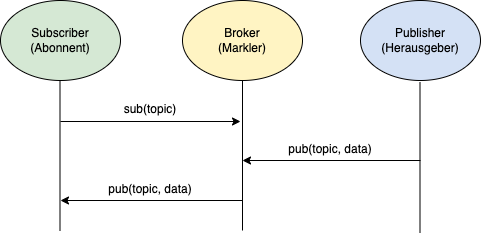
\includegraphics[width=12cm,height=12cm,keepaspectratio]{images/sub-model.drawio.png}
                \caption{Themenbasiertes Pub/Sub Kommunikationsmodell \cite{Hunkeler2008}}
                \label{pic:pub-sub-model}
            \end{figure}
            \\
            Dieses Prinzip ist die Grundlage des \acs{MQTT}-Protokolls. Im Folgenden wird ein Beispiel aufgezeigt, welches 
            die Kommunikation über das Publish/Subscribe Modell darstellt.
            
            \subsubsection*{Beispiel}
            \label{subsubsec:pubsub-example}
            Damit am Beispiel der Steuerzentrale, die im Rahmen dieser Arbeit konzipiert und prototypisch implementiert wird, 
            ein Prozess gestartet werden kann, müssen bestimmte Ereignisse durch \acs{MQTT}-Nachrichten eintreten. Das hier 
            verwendete Beispiel ist das Öffnen einer Büroeingangstür. Hierbei wird von einem Relais an der Tür, welches das 
            Türschloss steuert, eine Nachricht an den \textit{Broker} herausgegeben:
            \\
            \begin{lstlisting}[language=Java, frame=lines, xleftmargin=\parindent, style=algoBericht, label={code:pubmqtt}, captionpos=b, caption={Erzeugung und Veröffentlichung einer Nachricht}]
                publish -topic: Buero/Tuer/Zustand -message: "offen"
            \end{lstlisting}
            Diese Nachricht wird von der Steuerzentrale konsumiert und weiterverarbeitet. Damit der Informationskanal (topic) 
            über die Steuerzentrale verfügbar ist, muss dieser Kanal konsumiert werden: 
            \\
            \begin{lstlisting}[language=Java, frame=lines, xleftmargin=\parindent, style=algoBericht, label={code:submqtt}, captionpos=b, caption={Empfang und Konsum einer Nachricht}]
                subscribe -topic: Buero/Tuer/Zustand
            \end{lstlisting}
            Mit der empfangenen Nachricht kann dann über die Steuerzentrale ein Prozess, welcher vorab als Regel implementiert wurde, ausgelöst werden, 
            beispielsweise eine Durchsage im Büro.
    \pagebreak
    \subsection{AMQP}
    \label{subsec:amqp}
        Das \ac{AMQP}-Protokoll ist ebenso ein leichtgewichtiges \acs{MtoM}-Protokoll, welches im Jahre 2003 von John O\'Hara JPMorgan Chase 
        in London, Großbritannien, entwickelt wurde \cite{Naik2017}. Der Fokus dieses Protokolls liegt auf der Unternehmens-Messaging-Ebene. 
        Es wird hohen Wert auf die Zuverlässigkeit, Sicherheit, Bereitstellung und Interoperabilität der Kommunikation gelegt. \acs{AMQP} 
        unterstützt neben der Publish/Subscribe- auch die Request/Response Architektur. Es bietet eine Bandbreite an 
        Funktionen im Zusammenhang mit Messaging, wie z. B. Queuing, themenbasiertes Publish-and-Subscribe-Messaging, 
        flexibles Routing und Transaktionen \cite{Naik2017}. Das Kommunikationsmodell nach dem \acs{AMQP} Standard erfordert, dass der 
        Herausgeber (publisher) oder der Empfänger (subscriber) einen \textit{Austausch (exchange)} mit einem bestimmten Namen generiert 
        und diesen dann sendet \cite{Naik2017}. Die beiden Komponenten, Empfänger und Herausgeber, nutzen den Namen zum Austausch und zum 
        Verbindungsaufbau. Der Empfänger erstellt darauf eine Warteschlange (queue) und hängt diese an den Austausch an. Nachrichten, die 
        über diese Verbindung ausgetauscht werden, müssen über einen gesonderten Prozess (binding) mit der Warteschlange abgeglichen werden 
        \cite{Naik2017}.
        \\ 
        Das binäre Protokoll \acs{AMQP} erfordert einen Header von acht Byte mit Nachrichtennutzlasten. Die Größe der Nachricht ist abhängig 
        von dem Broker bzw. dem Server. Die verbindungsorientierte Kommunikation von \acs{AMQP} baut auf dem Standard-Transportprotokoll 
        \acs{TCP} auf. Durch das \acs{TLS}/\acs{SSL}-Protokoll wird die Kommunikationssicherheit gewährleistet. Ein Wesensmerkmal des \acs{AMQP} 
        Kommunikationsmodells ist die Zuverlässigkeit \cite{Naik2017}. 
        \\
        \linebreak
        Der direkte Vergleich der beiden Protokolle, \acs{MQTT} und \acs{AMQP}, ist dem Anhang (\ref{appendix:mqtt-amqp}) beigefügt.
        \\
        \linebreak
        Neben den beiden aufgeführten Kommunikationsmodellen gibt es noch weitere, darunter das klassische \ac{HTTP} und das \ac{COAP}, die allerdings 
        im Rahmen dieser Arbeit nicht weiter ausgeführt werden. 
        \\
        \linebreak
        Der Fokus liegt in dieser Arbeit auf dem \acs{MQTT}-Protokoll. 
